\begin{comment}
	\pagebreak
\end{comment}

\section{Auto-regressive Models}

\textbf{Regressive Property:} $x_t = b_0 + b_1 x_{t-1} + b_2 x_{t-2}$

\textbf{Sequence Model:} $p(x) = \prod^N p(x_i | x_1,..,x_{i-1}) = \prod p(x_i | x_{<i})$\\
\begin{comment}
	We are trying to estimate a distribution here.\\
	\Note{Sequence models trivially fulfill the regressive property}\\
\end{comment}

\textbf{Believe Net:} $\whx_i = p(x_i = 1 | x_{<i}) = Ber(\sigma(\sum_1^{i-1} w_j^i x_j + w_0^i)$
\begin{comment}
	In this fully visible sigmoid belief network, the value of the next element is modelled as a Bernoulli variable.\\
	\Note{The weight Matrix $W \in \R^{n \times n}$ is triangular.}\\ 
	Element $i$ at row j contains $w_i^j$, describing weight of $x_i$ when calculating $\whx_j$.
	
	\begin{Figure}
 		\centering
 		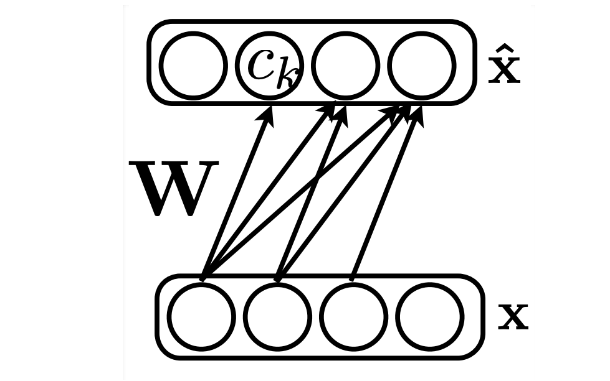
\includegraphics[width=.7\linewidth]{graphic/ar-fvsbNet}
 		\captionof{figure}{AR Fully Visible Sigmoid Belief Network}
	\end{Figure}
\end{comment}

\textbf{NADE:} $h_i = \sigma(b + \sum^{i-1} w_j x_j)$ (in $O(H)$, update in $O(1)$)\\
$\whx_i = p(x_i=1| x_{<i}) = \sigma(c_i + V_i h_i)$ ($N$ times $\Rightarrow$ total $O(NH)$)\\
\begin{comment}
	The difference to FVSB-Net is that the weights are shared.
	Therefore, the number of weights is in $\BigO(n)$.\\
	\Note{$b + W_{<i+1} x_{<i+1} = b + W_{<i} x_{<i} + W_{i+1} x_{i+1}$ in $\BigO(1)$} \\
	
	\begin{Figure}
 		\centering
 		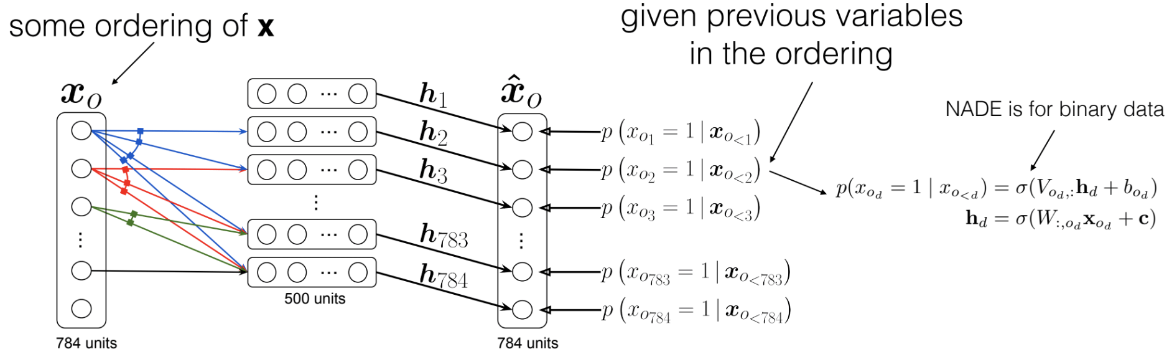
\includegraphics[width=\linewidth]{graphic/ar-nade}
 		\captionof{figure}{AR NADE Schema}
	\end{Figure}
\end{comment}

\textbf{PixelRNN:} $p(x) = \prod^{N^2} p(x_i | x_{<i}) = p(x_{i,R} | x_{<i}) p(x_{i,G} | x_{<i}, x_{i,R}) p(x_{i,B} | x_{<i}, x_{i,R}, x_{i,G})$\\
RNN's are autoreg. from nature: $h_t$ summarises inputs $<t$\\
\begin{comment}
	Learning and generation is slow, because of the explicit pixel dependencies from the pixel ordering.\\
	If we use a LSTM for example, $h_{i,j} = f(h_{i-1,j}, h_{i,j-1}, p_{i,j})$, e.g. no parallelization in training, neither in prediction, can be made. 
	It is very slow, but LSTM and RNN can capture long-term dependencies very well.\\
	
	\begin{Figure}
 		\centering
 		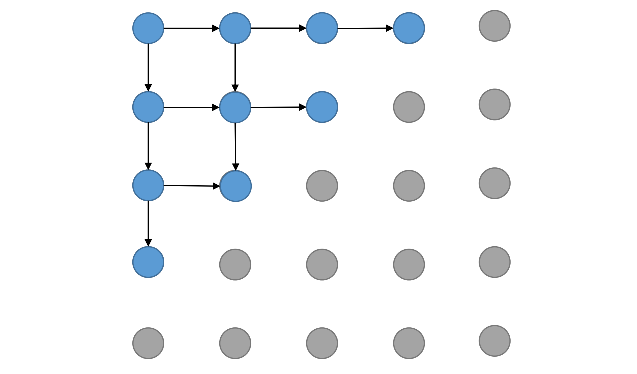
\includegraphics[width=\linewidth]{graphic/ar-pixelRNN}
 		\captionof{figure}{AR PixelRNN dependencies}
	\end{Figure}
\end{comment}

\textbf{PixelCNN:} Use conv + mask, parallelize training, blind spot\\
\begin{comment}
	\Note{Generation is still sequential}\\
	\textbf{Summary:}\\
	Pros are the explicit likelihood p(x) and good evaluation metric through LL of training data.\\
	Cons are slow generation\\
\end{comment}

\textbf{WaveNet:} dilated convolution for large scale temp. dependencies\\
\begin{comment}
	The issue with sound is that the frequency is at $\sim$ 16'000 samples/second.\\
	To capture speach, convolution must have a very large receptive field.\\
	
	\begin{Figure}
 		\centering
 		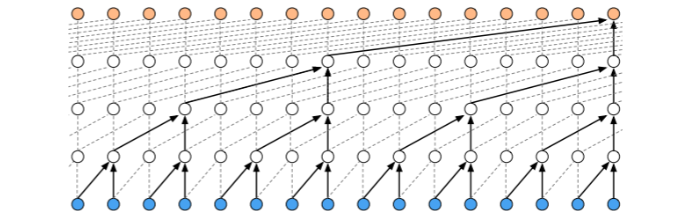
\includegraphics[width=\linewidth]{graphic/ar-wavenet-dilution}
 		\captionof{figure}{AR WaveNet long term dependencies}
	\end{Figure}
\end{comment}

\textbf{Dilated Conv:} exponential receptive field size increase\\
\begin{comment}
	\begin{Figure}
 		\centering
 		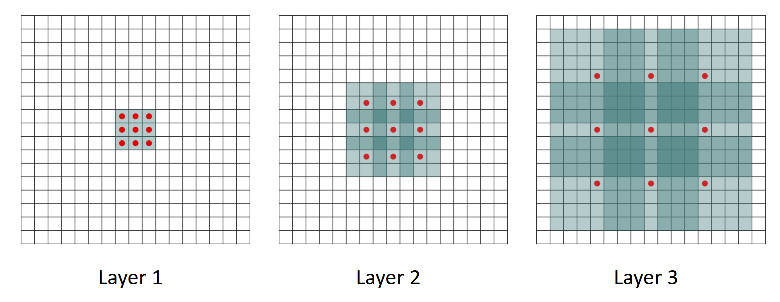
\includegraphics[width=\linewidth]{graphic/ar-receptive-field-1}
 		\captionof{figure}{Dilated Conv: Receptive field increase 1}
	\end{Figure}
	\begin{Figure}
 		\centering
 		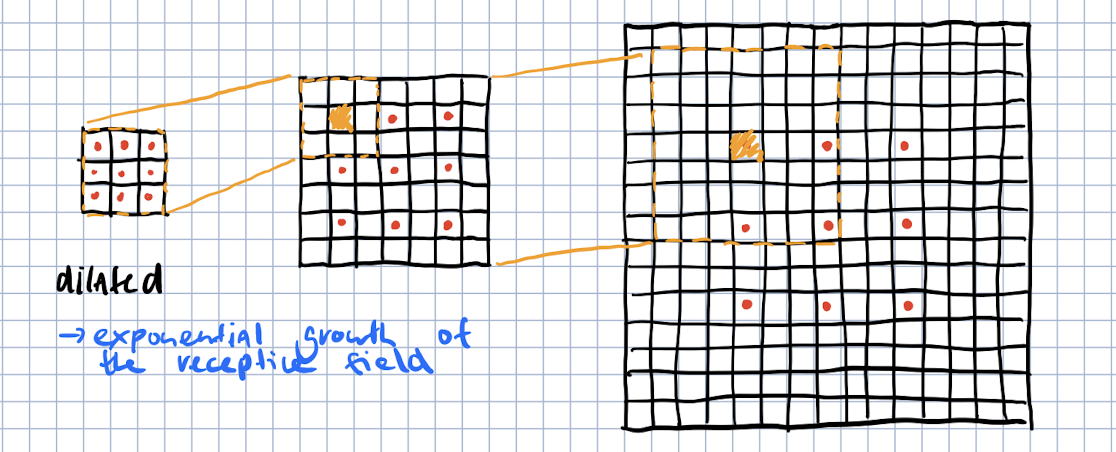
\includegraphics[width=\linewidth]{graphic/ar-receptive-field-2}
 		\captionof{figure}{Dilated Conv: Receptive field increase 2}
	\end{Figure}
\end{comment}

\textbf{Self-Attention:} $K=XW_K, V=XW_V, Q=x_{t}W_Q (\in \R^{D}),\\ 
X\in \R^{T\times D}, W\in \R^{D\times D}, \alpha = softmx(QK^T/\sqrt{D}), x_{t+1} = \alpha V$\\
$X = softmax(\frac{(W_QX)(W_KX)^T}{\sqrt{D}} + M) (W_VX)$\\
\begin{comment}
	\textbf{RNN:} $h_t = g(x_{t-1}, h_{t-1})$, $x_t = f(x_{t-1}, h_t)$.
	Learns to encode relevant information for future steps and maintains long-term temporal relations.\\
	\textbf{CNN:} $x_t = f(x_{t-1}, x_{t-2}, ..,x_{1})$.
	Learns to aggregate past information for the next step.\\
	\textbf{Self Attention:} $x_t = f(x_{t-1}, x_{t-2}, ..,x_{1})$.
	Learns to identify relevant information for the next step.\\
	Very expressive, but computationally complex. Attention is a quadratic operation.
	
	\begin{Figure}
 		\centering
 		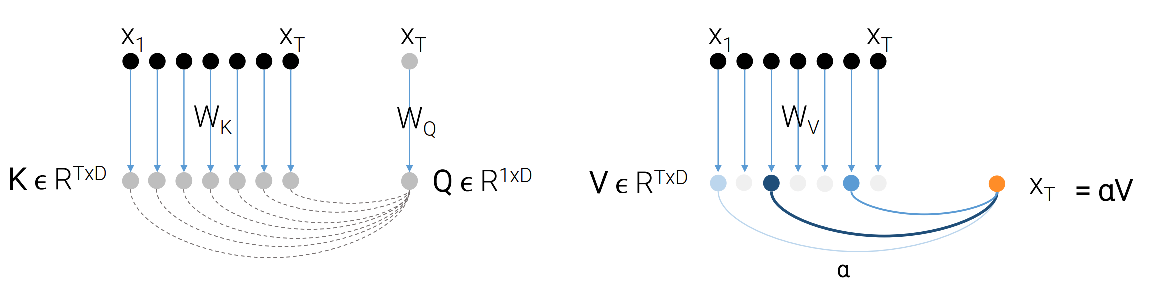
\includegraphics[width=\linewidth]{graphic/ar-self-attention}
 		\captionof{figure}{AR Self-attention}
	\end{Figure}
\end{comment}





